%%% -*-LaTeX-*-

\chapter[Rigorous Roundoff Error Analysis of Probabilistic Floating Point Computations]{Rigorous Roundoff Error Analysis of Probabilistic Floating Point Computations}
\label{sec:cav}
Reprinted from Proceedings of the 33rd International Conference on Computer-Aided Verification (CAV), pages 626-650, May 2021: "Rigorous Roundoff Error Analysis of Probabilistic Floating-Point Computations" by G.~Constantinides, F.~Dahlqvist, Z.~Rakamari\'c and R.~Salvia. Reprinted by permission.\\
https://doi.org/10.1007/978-3-030-20652-9\_25

\setupuuchapterbib
\uudummysection {Introduction}                              		{1}

\uudummysection {Overview Through an Application}					{3}
\uudummyfigure {Probabilistic correction of GPS coordinates from [2]: radius is Rayleigh distributed, angle is uniformly distributed.}           	{3}
\uudummytable {Roundoff error analysis for the probabilistic latitude correction of (1)} 															{4}

\uudummysection {Preliminaries}       								{5}
\uudummysubsection {Floating-Point Arithmetic}               	{5}

\uudummysubsection {Probability Theory}								{6}

\uudummysection {Distribution of Floating-Point Roundoff Errors}	{8}
\uudummysubsection {Derivation of the Distribution of Rounding Errors}               															{8}
\uudummyfigure {Error distribution versus the corresponding empirical error distributions, clockwise from topleft: (i) Eq. (6) for Unif(2, 4) 3 bit exponent, 4 bit significand, (ii) Eq. (6) for Unif(2, 4) in half-precision, (iii) Eq. (7) for Unif(7, 8) in single-precision, (iv) Eq. (7) for Unif(4, 5) in single-precision, (v) Eq. (7) for Unif(4, 32) in single-precision, (vi) Eq. (7) for Norm(0, 1) in single-precision.}																{10}
\uudummysubsection {High-Precision Case}               																							{10}
\uudummysubsection {Typical Distribution}						{11}
\uudummyfigure{Typical distribution.}								{11}
\uudummysubsection {Covariance Structure}						{11}
\uudummysubsection {Error Terms and P-Boxes}						{12}

\uudummysection {Symbolic Affine Arithmetic}						{12}

\uudummysection {Algorithm and Implementation}						{13}
\uudummysubsection {Probabilistic Model}							{13}
\uudummyfigure {Toolflow of PAF.}           						{14}
\uudummysubsection {Computing Probabilistic Ranges for Dependent Operands}																		{15}
\uudummysubsection {Computing Conditional Roundoff Error}																						{15}



\uudummysection {Experimental Evaluation}       					{16}

\uudummytable {Roundoff error bounds reported by PAF, PrAn, and FPTaylor given uniform (uni), normal (norm), and Laplace (exp) input distributions. We set the confidence interval to 99\% for PAF and PrAn, and mark the smallest reported roundoff errors for each benchmark in bold. Asterisk (*) highlights a difference of more than one order of magnitude between PAF and FPTaylor.} 															{17}

\uudummysection {Related Work}										{18}
\uudummysection {Conclusions and Future Work}						{19}
\uudummysection {References}										{21}
\uudummysection {Appendix A - Proofs}								{23}
\uudummysection {Appendix B - Implementation}						{32}
\uudummysection {Appendix C - Experimental Evaluation}				{33}


\uudummytable {Comparison between PAF, given uniform (uni), normal (norm) and exponential (exp) input distributions, and FPTaylor. The PAF columns report 99\% of the support of the output range distribution. The FPTaylor columns report the worst-case output ranges. The asterisk (*) highlights a difference of more than one order of magnitude between PAF and FPTaylor.} 							          						{33}



\uudummyfigure {CDFs of the range (left) and error (right) distributions for the benchmark train3 for uniform (top), normal (center), and exp (bottom)} 							          						{34}

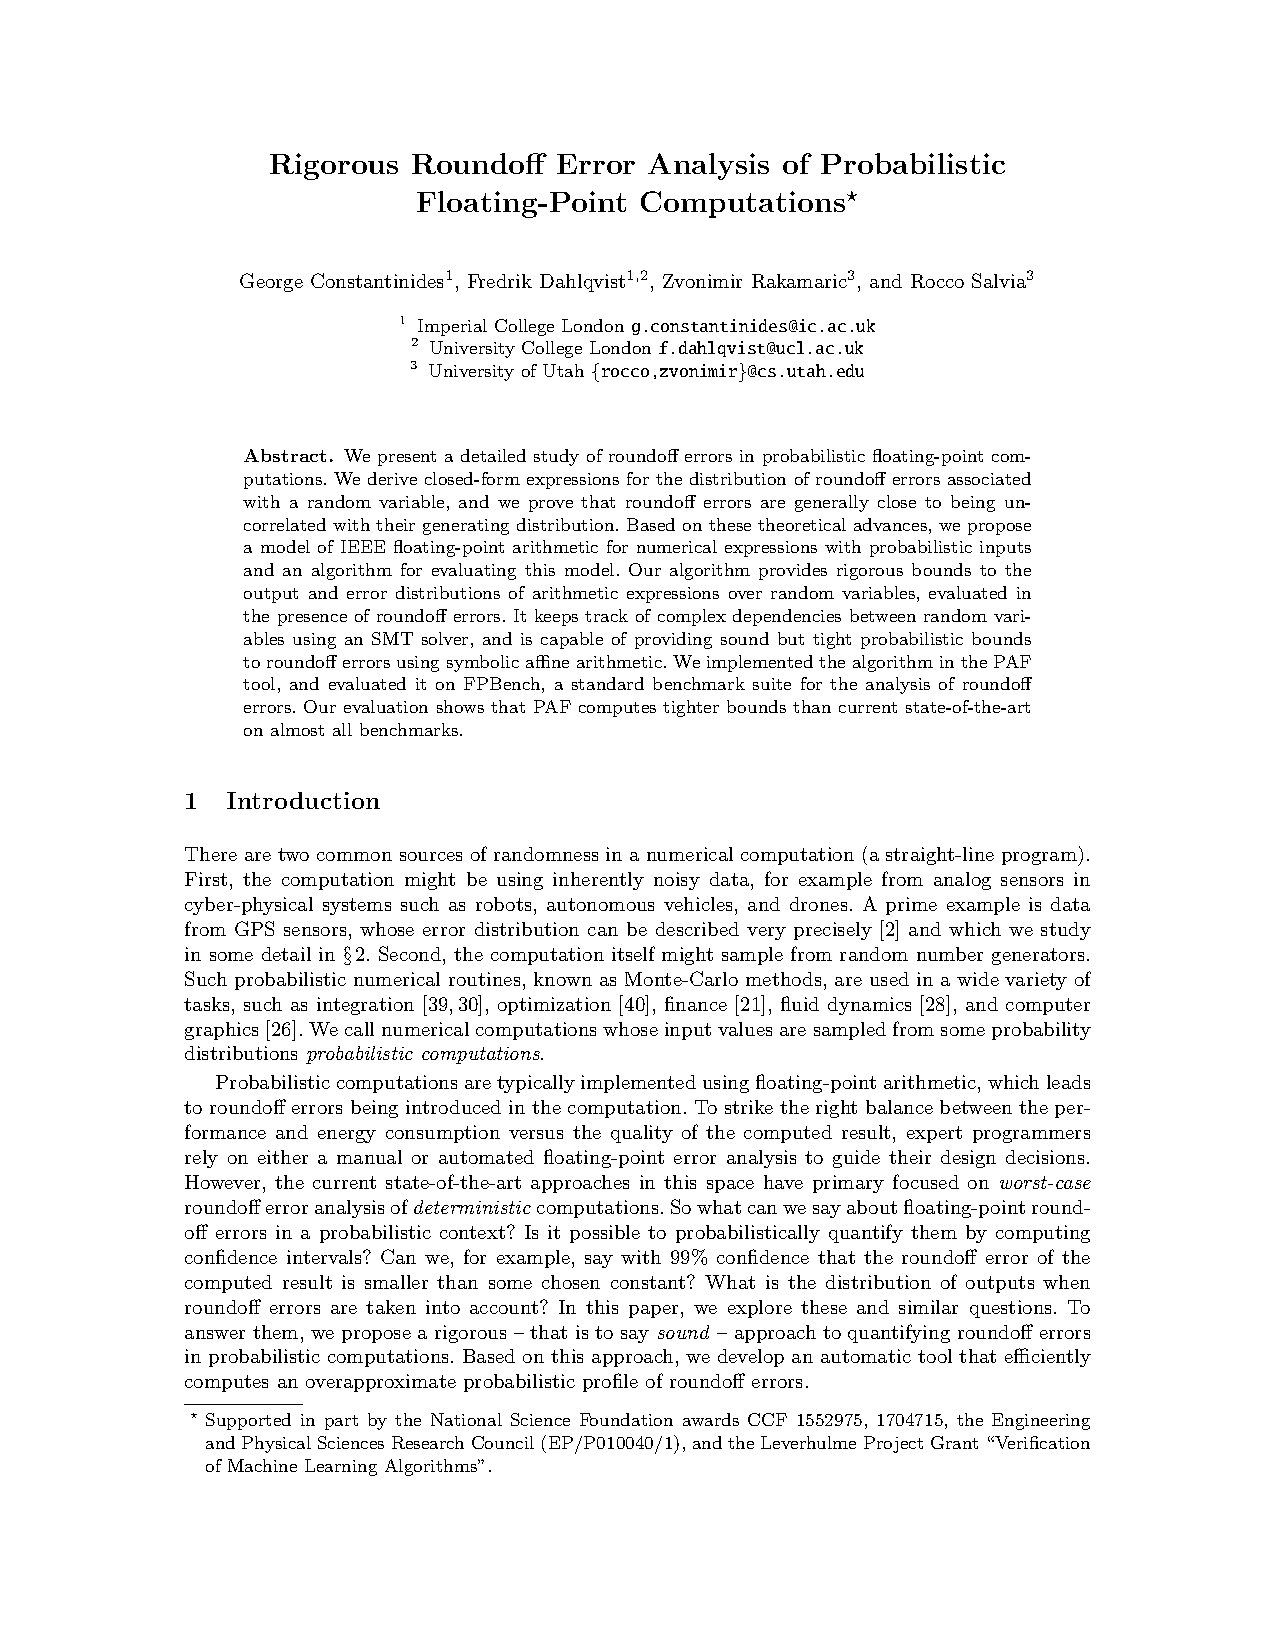
\includepdf[
pages = -,          % want all document pages
scale = 0.95,       % adjust to fit thesis page box
pagecommand = {\pagestyle{plain}} % bare page numbers
]{cav/main_long.pdf}

%\BibTeX{} entries themselves.
%\bibliographystyle{siam}
%\bibliography{\jobname}